\documentclass{standalone}
\usepackage[T1]{fontenc}
\renewcommand*\familydefault{\sfdefault} %%
\usepackage{sfmath}
\usepackage{pgfplots}

\begin{document}


\tikzset{every picture/.style={line width=0.75pt}} %set default line width to 0.75pt        

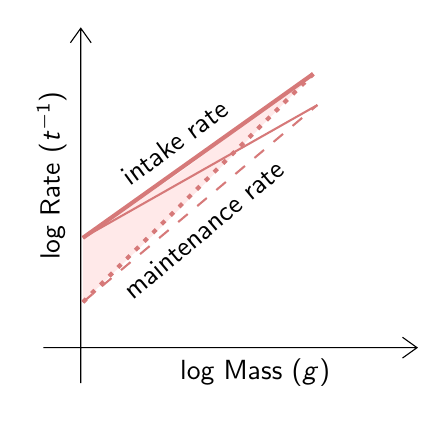
\begin{tikzpicture}[x=0.75pt,y=0.75pt,yscale=-1,xscale=1]
%uncomment if require: \path (0,300); %set diagram left start at 0, and has height of 300

%Shape: Polygon [id:ds30573961466433697] 
\draw  [draw opacity=0][fill={rgb, 255:red, 255; green, 233; blue, 233 }  ,fill opacity=1 ] (118,122) -- (183,74) -- (112.75,145) -- (72,184) -- (72,153) -- cycle ;
%Shape: Axis 2D [id:dp11951800865429041] 
\draw  (53,205.9) -- (233,205.9)(71,52) -- (71,223) (226,200.9) -- (233,205.9) -- (226,210.9) (66,59) -- (71,52) -- (76,59)  ;
%Straight Lines [id:da9694038502069455] 
\draw [color={rgb, 255:red, 214; green, 121; blue, 121 }  ,draw opacity=1 ][line width=0.75]    (72,153) -- (185,89) ;


%Straight Lines [id:da11732192728730761] 
\draw [color={rgb, 255:red, 214; green, 121; blue, 121 }  ,draw opacity=1 ][line width=0.75]  [dash pattern={on 4.5pt off 4.5pt}]  (72,184) -- (185,89) ;


%Straight Lines [id:da6895273087425773] 
\draw [color={rgb, 255:red, 214; green, 121; blue, 121 }  ,draw opacity=1 ][line width=1.5]  [dash pattern={on 1.69pt off 2.76pt}]  (72,184) -- (183,74) ;


%Straight Lines [id:da07284388810388731] 
\draw [color={rgb, 255:red, 214; green, 121; blue, 121 }  ,draw opacity=1 ][line width=1.5]    (72,153) -- (183,74) ;



% Text Node
\draw (57,123) node [rotate=-270] [align=left] {log Rate ($t^{-1}$)};
% Text Node
\draw (155,218) node  [align=left] {log Mass ($g$)};
% Text Node
\draw (130,149) node [rotate=-320] [align=left] {maintenance rate};
% Text Node
\draw (116,107) node [rotate=-323.84] [align=left] {intake rate};


\end{tikzpicture}
\end{document}